\documentclass[a4paper,14pt]{extreport}
\usepackage[utf8]{inputenc}
\usepackage[T2A]{fontenc}
\usepackage[russian]{babel}
\usepackage{eufrak}
% поля:
\usepackage[left=1cm, right=1cm, top=2cm, bottom=2cm]{geometry}
\linespread{1}
\usepackage{indentfirst} % отделять первую строку раздела абзацным отступом
\setlength\parindent{5ex}
\addto{\captionsrussian}{\renewcommand*{\contentsname}{Содержание}}
\usepackage[hidelinks]{hyperref} % гиперссылки в содержании
\usepackage{graphicx}
\usepackage{float}
\usepackage{amsmath}
\renewcommand*{\thesection}{\arabic{section}}

\usepackage{multirow}
\usepackage[normalem]{ulem}
\useunder{\uline}{\ul}{}

\usepackage{cmap}%позволяет копировать кириллицу из скомпилированного файла

% Глубина разделов, попадающих в содержание
\setcounter{tocdepth}{3}

\linespread{1.3} % настройка межстрочного интервала
\tolerance=1000 % настройка чувствительности вставки переносов
\hfuzz=0pt
\sloppy

\begin{document}
	
	\begin{titlepage}
		\begin{center}
			\large
			МИНИСТЕРСТВО ОБРАЗОВАНИЯ И НАУКИ\\ РОССИЙСКОЙ ФЕДЕРАЦИИ
			
			\textbf{Федеральное агентство по образованию}
			\vspace{0.5cm}
			
			УНИВЕРСИТЕТ ИТМО
			\vspace{0.25cm}
			
			Факультет компьютерных технологий и управления
			
			Кафедра систем управления и информатики
			\vfill
			
			
			Студент: Артемов Кирилл\\
			группа P4135\\
			Вариант №2\\
			\textsc{Лабораторная работа №3}\\[5mm]
			
			{\LARGE Построение дискретных генераторов задающих воздействий}
			\bigskip
			
		\end{center}
		\vfill
		
		\newlength{\ML}
		\settowidth{\ML}{«\underline{\hspace{0.7cm}}» \underline{\hspace{2cm}}}
		\hfill\begin{minipage}{0.4\textwidth}
			Преподаватель\\
			\underline{\hspace{\ML}} Ю.\,В.~Литвинов\\
			«\underline{\hspace{0.7cm}}» \underline{\hspace{2cm}} 2016 г.
		\end{minipage}%
		\bigskip
		
		\vfill
		
		\begin{center}
			Санкт-Петербург, 2016 г.
		\end{center}
	\end{titlepage}
\newpage

\section{Цель работы}

Ознакомление с принципами построения дискретных моделей внешних
воздействий – сигналов задания и возмущения.

\section{Порядок выполнения работы}

а) в соответствии с вариантом задания (таблица 1) построить математическую
модель командного генератора сигнала сканирования 
\begin{equation*}
	g(k) = A sin(\omega k T);
\end{equation*}

б) построить схемы моделирования дискретного генератора;

в) осуществить моделирование работы дискретного генераторов. На экран выводить
g(k);

г) Для уравнения (1) построить модель ВСВ дискретного ОУ и проделать пункты б)-в). Интервал дискретности выбрать равным 0,25. 
с
\begin{table}[H]
	\centering
	\caption{Параметры командного генератора сигналов}
	\label{my-label}
	\begin{tabular}{|c|c|c|c|}
		\hline
		№ & T, c & A     & $\omega$ \\ \hline
		2 & 0.2  & -1.42 & 0.02     \\ \hline
	\end{tabular}
\end{table}

Возмущающее воздействие:
\begin{equation}
	2 sin(2 k T) + 3 cos(5 k T)
\end{equation}

\section{Ход работы}

а) построение математической модели командного генератора

Дискретная модель внешнего воздействия описывается в пространстве
состояний системой разностных уравнений:

\begin{align*}
\begin{cases}
	\xi(k+1) &= \Gamma \xi(k)\\
g(k) &= H\xi(k)
\end{cases}
\end{align*}
где $\xi(k)$ -- n-мерный векторк состояния дискретного командного генератора, $\Gamma$ -- $n \times n$ матрица динамических свойств дискретного генератора, $H$ -- $1 \times n$ матрица выхода модели.


Найдем первую и вторую разности для $g(k)$:
\begin{align}
	g(k+1) = A sin(\omega (k +1) T) = A sin(\omega k T) cos(\omega T) + A cos(\omega k T) sin(\omega T);
\end{align}
Учитывая $A sin(\omega k T) = g(k)$, получим:
\begin{align}
g(k+1) = A sin(\omega (k +1) T) = g(k) cos(\omega T) + A cos(\omega k T) sin(\omega T);\\
g(k+2) = g(k+1) cos(\omega T) + sin(\omega T) [A cos(\omega k T) cos(\omega T) + A sin(\omega k T ) sin(\omega T)].
\end{align}
Выразим из (6):
\begin{align}
	A cos(\omega k T) = \frac{g(k+1) - g(k) cos(\omega T)}{sin(\omega T)}
\end{align}
Подставим (8) в (7) и, упростив, получим:
\begin{align}
	g(k+2) = 2 g(k+1) cos(\omega T) -g(k).
\end{align}

Пимем в качестве вектора состояния следующие уравнения:
\begin{align}
\xi_1(k) &= g(k);\\
\xi_2(k) &= \xi_1(k+1) + g(k+1);\\
\xi_3(k) &= \xi_2(k+1) + g(k+2).
\end{align}

Составив из полученных уравнений систему, получим модель в пространстве состояний:
\begin{equation}
	\begin{cases}
	\begin{bmatrix}
	\xi_1(k+1) \\
	\xi_2(k+1)
	\end{bmatrix}
	&=\begin{bmatrix}
	0&1\\
	-1& 2 cos(\omega T)
	\end{bmatrix}
	\begin{bmatrix}
	\xi_1(k)\\
	\xi_2(k)
	\end{bmatrix}
	\\
	g(k) &= \begin{bmatrix}
	1& 0
	\end{bmatrix}
	\begin{bmatrix}
	\xi_1(k)\\
	\xi_2(k)
	\end{bmatrix}
	\end{cases}
\end{equation}

с начальными условиями:
\begin{align}
	\xi_1(0) &= A sin(0) = 0;\\
	\xi_2(0) &= A sin(0) cos(\omega T) + A cos(0) sin(\omega T) = A  sin(\omega T).
\end{align}

Учитывая параметры командного генератора из таблицы 1, получим:
\begin{equation}
\begin{cases}
\begin{bmatrix}
\xi_1(k+1) \\
\xi_2(k+1)
\end{bmatrix}
&=\begin{bmatrix}
0&1\\
-1& 1.9999
\end{bmatrix}
\begin{bmatrix}
\xi_1(k)\\
\xi_2(k)
\end{bmatrix}
\\
g(k) &= \begin{bmatrix}
1& 0
\end{bmatrix}
\begin{bmatrix}
\xi_1(k)\\
\xi_2(k)
\end{bmatrix}
\end{cases}
\end{equation}

\begin{align}
\xi_1(0) &= 0;\\
\xi_2(0) &= -0.0056800
\end{align}

б) схема моделирования полученного генератора

\begin{figure}[H]
	\center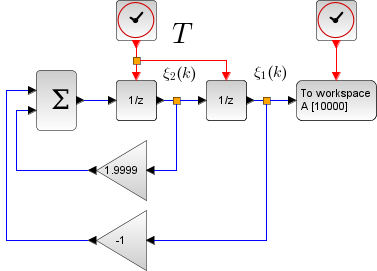
\includegraphics[width=0.5\linewidth]{a.png}
	\caption{Схема моделирования дискретного генератора}
	\label{fig:scr1}
\end{figure}

в) моделирование дискретного генератора

\begin{figure}[H]
\begin{minipage}[h]{0.49\linewidth}
	\center{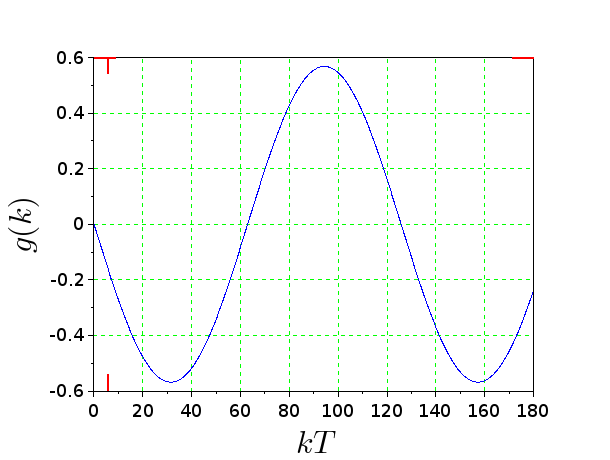
\includegraphics[width=1\linewidth]{a_res1.png} \\ а)}
\end{minipage}
\hfill
\begin{minipage}[h]{0.49\linewidth}
	\center{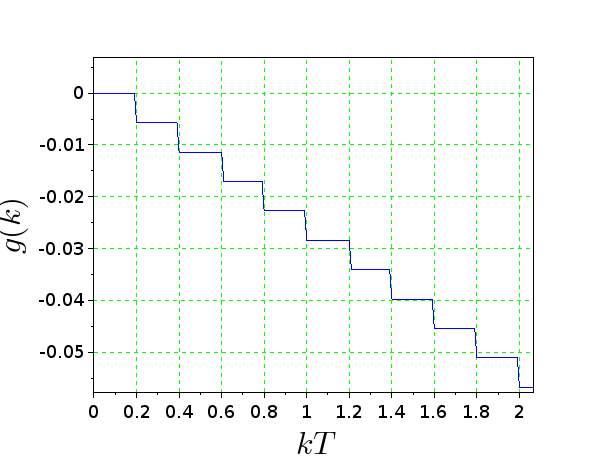
\includegraphics[width=1\linewidth]{a_res2.png} \\ б)}
\end{minipage}
\caption{Результаты моделирования в течение : a) 180 сек.; б) 2 сек.}
\label{ris:image1}\end{figure}

г) построение модели ВСВ дискретного объекта управления

В соответствии с вариантом, объект управления описывается выражением:
\begin{equation}
	y(k) = 2 sin(2kT) + 3 sin(5kt)
\end{equation}
где $T = 0.25 сек.$ -- интервал дискретности равный.
	
Для упрощения задачи расчета представим ОУ в виде суммы двух составляющих:
\begin{equation}
y(k) = y_1(k) + y_2(k) = 2 sin(2kT) + 3 cos(5kT)
\end{equation}
где 
\begin{equation}\label{eq1}
y_1(k) = 2 sin(2kT)
\end{equation}
\begin{equation}\label{eq2}
y_2(k) = 3 cos(5kT)
\end{equation}

Построим модель ВСВ для (\ref{eq1}).
Найдем первую и вторую разности для $y_1(k)$:
\begin{align}\label{eq3}
y_1(k+1) = 2 sin(2 (k +1) T) = 2 sin (2kT) cos (2T) + 2 cos(2kT) sin(2T)
\end{align}
Учитывая $2 sin(2 k T) = y_1(k)$, получим:
\begin{align}\label{eq5}
y_1(k+1) = y_1(k) cos (2T) + 2 cos(2kT) sin(2T)
\end{align}
Выразим из (\ref{eq3}):
\begin{align}\label{eq4}
2 cos(2 k T) = \frac{y_1(k+1) - y_1(k) cos(2 T)}{sin(2 T)}
\end{align}
Подставим (\ref{eq4}) в (\ref{eq5}) и, упростив, получим:
\begin{align}
y_1(k+2) = 2 y_1(k+1) cos(2 T) - y_1(k).
\end{align}

Пимем в качестве вектора состояния следующие уравнения:
\begin{align}
\xi_{11}(k) &= y_1(k);\\
\xi_{12}(k) &= \xi_{11}(k+1) + y_1(k+1);\\
\xi_{13}(k) &= \xi_{12}(k+1) + y_1(k+2).
\end{align}

Составив из полученных уравнений систему, получим модель в пространстве состояний:
\begin{equation}
\begin{cases}
\begin{bmatrix}
\xi_{11}(k+1) \\
\xi_{12}(k+1)
\end{bmatrix}
&=\begin{bmatrix}
0&1\\
-1& 2 cos(2 T)
\end{bmatrix}
\begin{bmatrix}
\xi_{11}(k)\\
\xi_{12}(k)
\end{bmatrix}
\\
y_1(k) &= \begin{bmatrix}
1& 0
\end{bmatrix}
\begin{bmatrix}
\xi_{11}(k)\\
\xi_{12}(k)
\end{bmatrix}
\end{cases}
\end{equation}

с начальными условиями:
\begin{align}
\xi_{11}(0) &= 2 sin(0) = 0;\\
\xi_{12}(0) &= 2 sin(0) cos(2T) + 2 cos(0) sin(2 T) = 2  sin(2 T).
\end{align}

Для заданного $T = 0.25 сек.$, имеем:
\begin{equation}
\begin{cases}
\begin{bmatrix}
\xi_{11}(k+1) \\
\xi_{12}(k+1)
\end{bmatrix}
&=\begin{bmatrix}
0&1\\
-1& 1.7551
\end{bmatrix}
\begin{bmatrix}
\xi_{11}(k)\\
\xi_{12}(k)
\end{bmatrix}
\\
y_1(k) &= \begin{bmatrix}
1& 0
\end{bmatrix}
\begin{bmatrix}
\xi_{11}(k)\\
\xi_{12}(k)
\end{bmatrix}
\end{cases}
\end{equation}

\begin{align}
\xi_{11}(0) &= 0;\\
\xi_{12}(0) &= 0.9589
\end{align}

Проделывая тоже для $y_2$, получим следующую модель ВСВ:
\begin{equation}
\begin{cases}
\begin{bmatrix}
\xi_{21}(k+1) \\
\xi_{22}(k+1)
\end{bmatrix}
&=\begin{bmatrix}
0&1\\
-1 & 2 cos(5T)
\end{bmatrix}
\begin{bmatrix}
\xi_{21}(k)\\
\xi_{22}(k)
\end{bmatrix}
\\
y_2(k) &= \begin{bmatrix}
1& 0
\end{bmatrix}
\begin{bmatrix}
\xi_{21}(k)\\
\xi_{22}(k)
\end{bmatrix}
\end{cases}
\end{equation}

с начальными условиями:
\begin{align}
\xi_{21}(0) &= 3 cos(0) = 3;\\
\xi_{22}(0) &= 3 cos(0) cos(5T) - 3 sin(0) sin(5 T) = 3 cos(5T)
\end{align}

При подстановке интервала дискретности, получим:
\begin{equation}
\begin{cases}
\begin{bmatrix}
\xi_{21}(k+1) \\
\xi_{22}(k+1)
\end{bmatrix}
&=\begin{bmatrix}
0&1\\
-1  & 0.6307
\end{bmatrix}
\begin{bmatrix}
\xi_{21}(k)\\
\xi_{22}(k)
\end{bmatrix}
\\
y_2(k) &= \begin{bmatrix}
1& 0
\end{bmatrix}
\begin{bmatrix}
\xi_{21}(k)\\
\xi_{22}(k)
\end{bmatrix}
\end{cases}
\end{equation}

с начальными условиями:S
\begin{align}
\xi_{21}(0) &= 	3;\\	
\xi_{22}(0) &= 0.9459
\end{align}

\begin{figure}[H]
	\center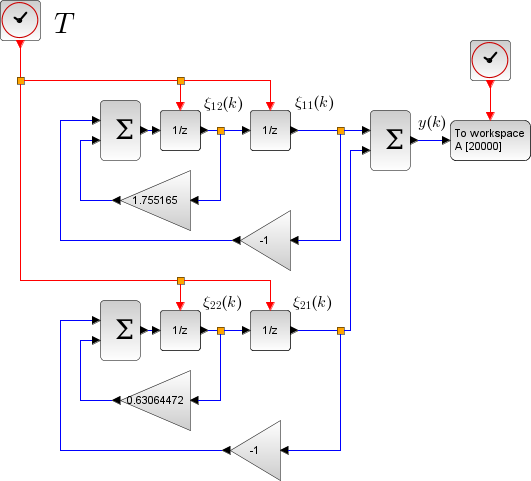
\includegraphics[width=0.68\linewidth]{b.png}
	\caption{Схема моделирования дискретного объекта}
	\label{fig:scr1}
\end{figure}

\begin{figure}[H]
	\center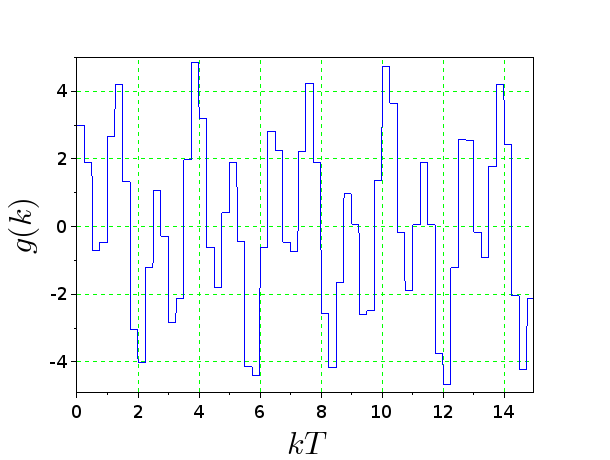
\includegraphics[width=0.7\linewidth]{b_res.png}
	\caption{Результаты моделирования дискретного объекта}
	\label{fig:scr1}
\end{figure}

\section*{Вывод}
В ходе работы было произведено ознакомление с принципами построения дискретных моделей внешних воздействий. Методики построения аналогичны непрерывным системам (методу последовательного дифференцирования, дискретный аналог – метод последовательного взятия разностей).

\end{document}
